\section{Experiments}
\label{sec:experiments}

\subsection{Setup}

We evaluate the framework on CPU and GPU traces collected from older GPT-style models and newer quantized instruct families. The strongest modern-family evidence comes from dense context sweeps on \texttt{Qwen2.5-1.5B}, \texttt{Qwen3-8B}, and \texttt{SmolLM2-1.7B}, together with an additional \texttt{Phi-3.5-mini} validation and targeted 8-bit robustness points on \texttt{Qwen2.5-1.5B} and \texttt{SmolLM2-1.7B}. Across the current artifact set, the main analysis covers 34 workload points. We report speedup relative to GPU-only execution under the virtual backend. Our primary realistic baselines are \texttt{online\_predictor}, \texttt{adaptive\_feature}, and \texttt{kv\_regime}; \texttt{oracle} serves only as an upper bound. The current setup is still limited in runtime and model breadth, so the paper should be read as a focused characterization study rather than as a broad serving-scale benchmark. While the current workload set is limited in size, our goal is not to establish universal thresholds, but to demonstrate the existence and consistency of regime-dependent behavior across representative modern families.

\subsection{Backend Transparency and Sensitivity}

The largest methodological risk in this paper is over-interpreting a virtual backend. We therefore make the backend explicit. \Cref{tab:backend-measured-modeled} separates trace-measured, trace-derived, and modeled quantities, while \Cref{tab:backend-params} lists the default parameters and their provenance. The most important anchor is that measured trace latency is used directly as the GPU reference whenever available; the roofline terms are then used only to decompose that measured latency into compute- and memory-dominant shares before applying the virtual PIM rescaling. On the current workload set, measured latency coverage is complete ($1088/1088$ records overall, including $544/544$ attention and $544/544$ MLP records), so the roofline fallback is not driving the main experiments.

The sensitivity analysis is defensive but important. Conservative, default, and optimistic virtual-PIM presets change absolute speedups, but the canonical weak cases remain weak and the canonical long-context positive cases remain positive. Across the preset study, online positive fraction moves from $0.50$ (conservative) to $0.75$ (default/optimistic), while delayed-onset families remain delayed and early-positive families remain early-positive in first-positive context. We therefore treat the backend as a transparent what-if model whose main value lies in preserving regime ordering, onset ordering, and relative decision-signal comparisons rather than exact numerical speedup claims.

\subsection{Negative Results Matter}

A key result of this study is that virtual PIM value is not automatic. \Cref{fig:negative-cases} shows this as a distribution rather than as a handful of cherry-picked bars. The left panel shows a clear mass of workloads near $\online = 1.0\times$, while the right panel shows that only $4/11$ short-context workloads are online-positive. The fraction rises to $9/9$ for mid-context workloads and $14/14$ for long-context workloads.

These negative results are important because they improve credibility. Rather than showing gains everywhere, the framework separates weak and positive regimes at the workload-distribution level, which makes the later positive-regime evidence more trustworthy. This also clarifies the main scientific claim: virtual PIM offload becomes interesting only after the decode stream enters the right operating regime, and short-context execution often fails to provide that signal.

\begin{figure}[t]
    \centering
    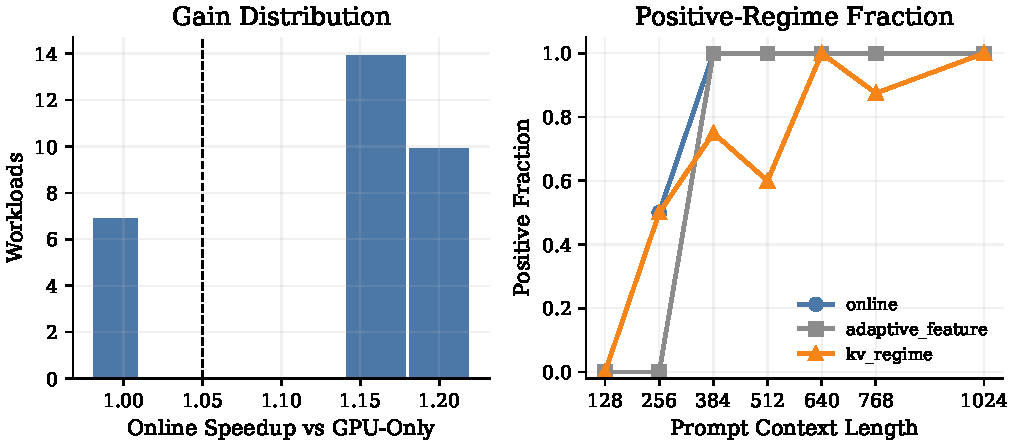
\includegraphics[width=0.95\linewidth]{figures/final_figures/paper_negative_cases.pdf}
    \caption{Distributional negative-result evidence. Left: workload-level distribution of realistic online gains. Right: positive-regime fraction versus context. Gains do not appear automatically, and short-context workloads are much more often weak.}
    \label{fig:negative-cases}
\end{figure}

\subsection{Context Governs Regime Entry}

\Cref{fig:context-transition} is the best-supported empirical result in the paper. It sharpens the regime transition using dense context sweeps instead of only coarse points such as 256, 512, and 768. The delayed-onset \texttt{Qwen2.5-1.5B} family transitions from weak to positive between 256 and 384 tokens, while \texttt{Qwen3-8B} and \texttt{SmolLM2-1.7B} become positive earlier, between 128 and 256 tokens. The extra \texttt{Phi-3.5-mini} validation remains positive at 256, 384, and 768 tokens, which shows that early-positive behavior is not isolated to a single family.

This result matters for two reasons. First, it supports a stronger claim than ``longer context helps'': in our current setup, context length is the clearest \emph{coarse} regime-entry variable. Second, it shows that onset is family-dependent rather than universal, which implies that a global rule such as ``offload attention after context 512'' is too coarse.

\subsection{KV-Related Signals Are Predictive, Not Causal}

\begin{figure}[t]
    \centering
    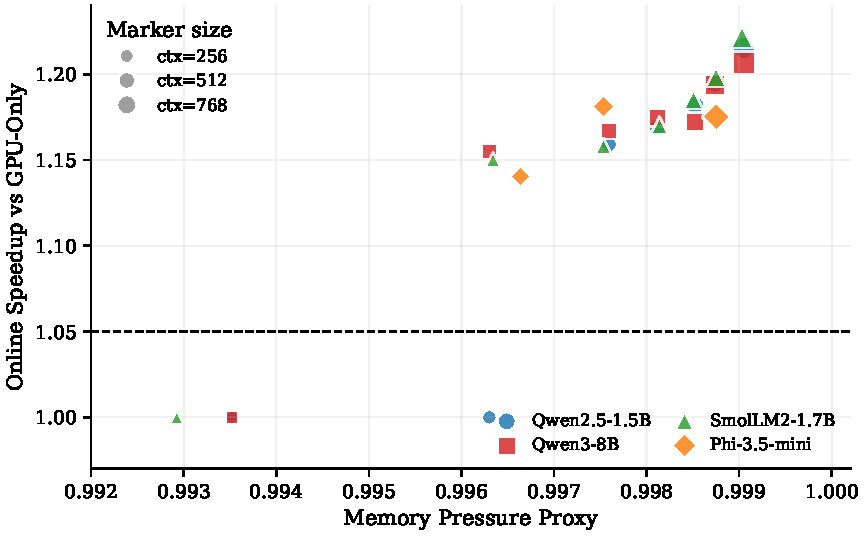
\includegraphics[width=0.95\linewidth]{figures/final_figures/paper_backbone_kv_pressure_vs_speedup.pdf}
    \caption{Higher memory-pressure proxy values align with positive online speedup across modern families. The figure is consistent with a KV-centered mechanism, but should be interpreted as predictive evidence rather than as causal proof.}
    \label{fig:kv-pressure}
\end{figure}

\begin{figure}[t]
    \centering
    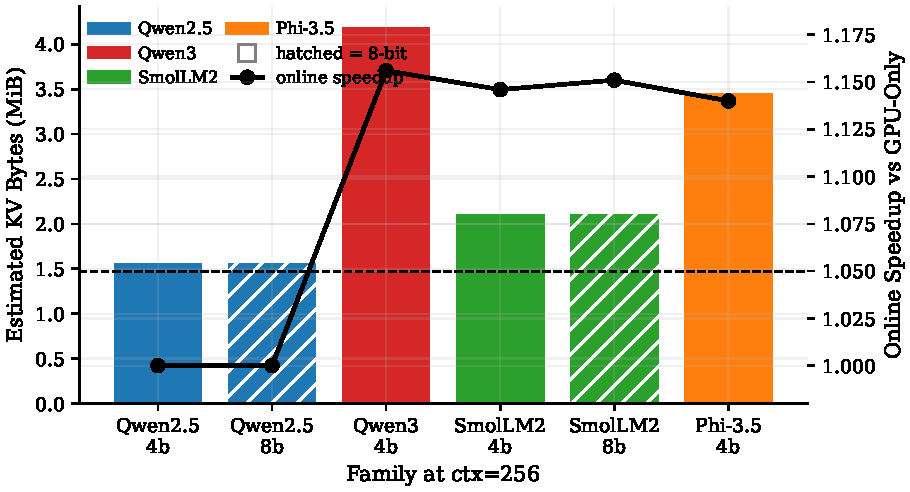
\includegraphics[width=0.95\linewidth]{figures/final_figures/paper_same_context_family.pdf}
    \caption{Same-context family comparison at $\ctx=256$. Delayed-onset \texttt{Qwen2.5} remains weak at the same context where \texttt{Qwen3}, \texttt{SmolLM2}, and \texttt{Phi-3.5} are already positive, and the stronger cases also carry larger KV-byte scale. This is supporting evidence for family-dependent onset under a fixed context rather than a causal proof.}
    \label{fig:same-context-family}
\end{figure}

The mechanism analysis strengthens the paper beyond a context-only observation, but we intentionally stop short of a causal claim. Across the focused GPU suite, higher memory-pressure proxy values align with positive online speedup more directly than attention share alone. This relationship is consistently visible across the representative families and contexts included in the dense-sweep suite. A same-context comparison at $\ctx=256$ also makes the family effect more concrete: delayed-onset \texttt{Qwen2.5} remains weak with much smaller KV-byte scale than early-positive \texttt{Qwen3}, \texttt{SmolLM2}, and \texttt{Phi-3.5} at the same context (\Cref{fig:same-context-family}). We therefore interpret the evidence as follows: the observed regime boundary is consistent with rising KV-cache-related pressure, and KV-related proxies are useful predictive correlates under the current backend.

This view also helps account for family-dependent onset. Different families can exhibit different KV-cache traffic profiles and attention behavior under similar context lengths, which means the same context value need not imply the same offload regime boundary.

\subsection{Held-Out Decision-Signal Study}

To test signal quality more directly, we built a workload-level classifier for positive-regime detection, where the label is whether the realistic online predictor reaches $\mathrm{speedup} > 1.05\times$. This classifier does not predict real-hardware benefit; it predicts positive-regime labels induced by the current virtual replay setup. We use it only to compare the relative informativeness of different signal families under a fixed backend definition.

We use class-weighted logistic regression with standardized features and a fixed decision threshold of $0.5$. We intentionally do not tune the decision threshold on this small dataset, because the goal is relative signal comparison rather than maximizing classifier accuracy. The study uses the same 34 workloads as the main analysis, with 5 family-held-out folds and 3 context-bucket-held-out folds. At the default $1.05\times$ label threshold, the dataset contains 27 positive workloads and 7 negative workloads. We compare five signal families: attention-only, context-only, context+attention, KV-only, and all-features.

The result is more nuanced than our earlier draft suggested. On family-held-out splits, context-only is the strongest coarse detector (F1 $=0.928 \pm 0.079$, false-positive rate $=0.000$), while attention-only is too permissive (positive recall $=0.757$, false-positive rate $=0.500$). The family-held-out F1 is slightly lower than in the earlier 30-workload draft because the added 8-bit robustness points lie close to the existing short-context and early-positive boundaries, which makes held-out family transfer modestly harder without changing the qualitative ordering. On context-bucket-held-out splits, the all-feature detector is strongest overall (F1 $=0.803 \pm 0.197$ versus $0.749 \pm 0.192$ for context-only), which suggests that KV-related signals are complementary decision aids rather than a standalone dominant mechanism. This ordering is not specific to logistic regression: a shallow decision tree preserves the same qualitative conclusion. Over thresholds from $1.01\times$ to $1.10\times$, the main qualitative ordering remains unchanged in this workload set, which reduces but does not eliminate threshold-sensitivity concerns.

We also evaluate a boundary-focused subset under the same backend definition. On 21 workloads with $1.00\times \le \online \le 1.18\times$, all-feature detectors reduce false positives relative to attention-only while remaining competitive with context-only in F1. This strengthens the practical interpretation of KV-related signals: they are most useful near the boundary, where coarse context cues alone are less decisive.

\begin{figure}[t]
    \centering
    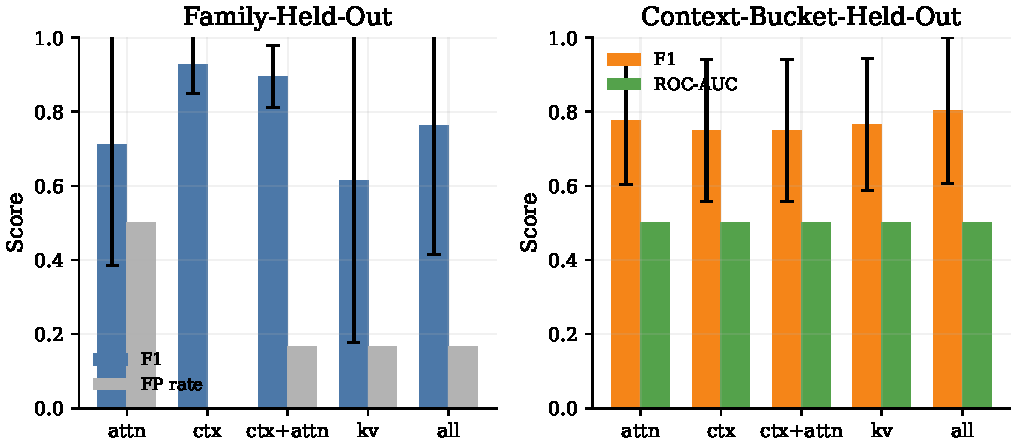
\includegraphics[width=0.95\linewidth]{figures/final_figures/paper_decision_signal_study.pdf}
    \caption{Held-out decision-signal study for workload-level positive-regime detection. Attention-only cues over-predict positive regimes, context is the strongest coarse predictor in the current setup, and all-feature detectors modestly improve context-bucket-held-out detection.}
    \label{fig:decision-signal-study}
\end{figure}

\subsection{Policy Case Study}

The policy results still matter, but they should be read as a focused case study rather than as proof of a universally best scheduler. A static attention heuristic is directionally useful and, in this 34-workload set, remains the strongest average-speedup baseline. Its weakness is not low average gain but permissiveness and limited interpretability at the regime boundary. The generic realistic policy \texttt{adaptive\_feature} is safer overall, but it misses several early-positive cases such as \texttt{Qwen3 @ ctx256}, \texttt{SmolLM2 @ ctx256}, and \texttt{Phi-3.5 @ ctx256}. This suggests that simple heuristics fail primarily due to regime misclassification rather than insufficient feature complexity. This figure is supporting evidence rather than the core backbone of the paper.

The more defensible message is that explicit KV-aware features can matter on some early-positive families. \texttt{kv\_regime} recovers \texttt{Qwen3 @ ctx256}, \texttt{SmolLM2 @ ctx256}, and \texttt{Phi-3.5 @ ctx256} without relying on oracle-like cost-model internals, but it is not uniformly dominant on every boundary point. We therefore frame this result as an existence proof that KV-aware decision features can be useful, not as a final scheduler contribution.

\begin{figure}[t]
    \centering
    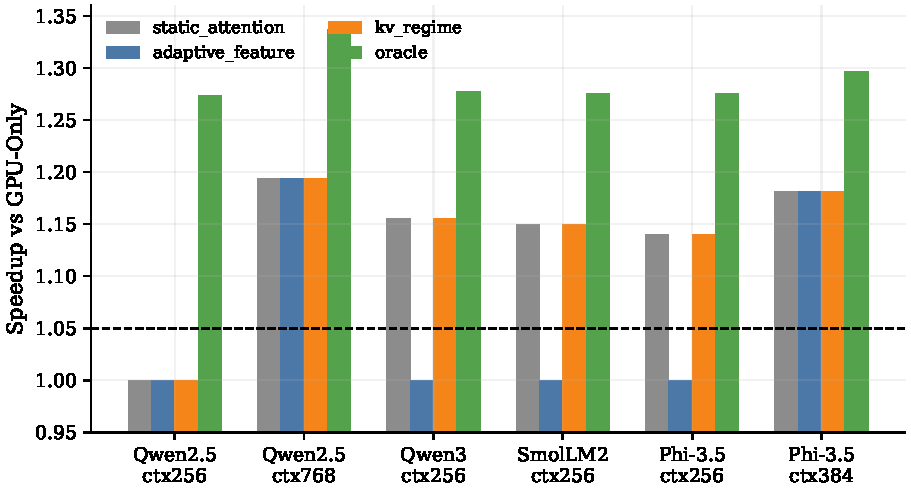
\includegraphics[width=0.95\linewidth]{figures/final_figures/paper_policy_comparison.pdf}
    \caption{Focused policy case study on selected early-positive workloads. KV-aware decision features can recover some early-positive cases that a generic realistic policy misses, but the figure should not be read as a universal ranking over all workloads.}
    \label{fig:policy-comparison}
\end{figure}

The policy comparison makes the paper's systems implication more concrete. Static attention offloading is often useful, but it does not capture why early-positive modern families differ from delayed-onset ones. The generic realistic policy \texttt{adaptive\_feature} is safer overall, but it still misses important early-positive points. In contrast, \texttt{kv\_regime} recovers several of these cases using only runtime-style KV-related signals and without direct oracle-like cost-model internals.

\subsection{Practical Method Translation}

To make the paper actionable, we translate the characterization results into a simple practical method: \texttt{context\_kv\_hysteresis}. The method uses context as a coarse gate, attention labeling only for candidate generation, KV-related signals for boundary refinement, and hysteresis thresholds to reduce switching. We keep the thresholds fixed and conservative rather than tuning them aggressively for average speedup.

\begin{table}[t]
\centering
\caption{Practical policy trade-offs over the 34-workload evaluation set. The added context+KV ablation isolates hysteresis itself: under the current trace granularity, hysteresis does not materially change aggregate behavior, so the practical gain comes primarily from conservative context+KV gating rather than from hysteresis alone.}
\label{tab:practical-policy}
\begin{tabular}{lccccc}
\toprule
Policy & Speedup & Oracle Regret & FP Rate & Missed-Pos. & Switches /100 \\
\midrule
GPU-only & 1.000 & 1.000 & 0.000 & 1.000 & 0.0 \\
Static attention & 1.181 & 0.359 & 0.000 & 0.500 & 0.0 \\
Context threshold & 1.132 & 0.557 & 0.000 & 0.662 & 0.0 \\
Adaptive feature & 1.132 & 0.557 & 0.000 & 0.664 & 0.7 \\
KV regime & 1.122 & 0.573 & 0.000 & 0.662 & 0.0 \\
Context+KV & 1.112 & 0.612 & 0.000 & 0.694 & 0.2 \\
Context+KV+hyst. & 1.112 & 0.612 & 0.000 & 0.694 & 0.2 \\
\bottomrule
\end{tabular}
\end{table}


\Cref{tab:practical-policy} shows the resulting trade-off. The proposed two-stage hysteresis policy achieves lower average speedup than the most aggressive baselines, especially \texttt{static\_attention}, but its role is different: it translates the paper's findings into a conservative practical detector with explicit control over missed-positive and switching behavior. The most informative comparison is against the same context+KV detector without hysteresis: this ablation isolates the stability effect itself. Under the current trace granularity, hysteresis does not materially change aggregate behavior, which means that the practical gain currently comes mostly from conservative context+KV gating rather than from hysteresis alone. We therefore present the method as a pragmatic detector template rather than as a new optimal scheduler.

\subsection{Batch and Robustness Are Defensive Evidence}

In the controlled \texttt{Qwen2.5-1.5B} batch sweep, batch appears weaker than context. Online speedup remains exactly $1.000\times$ across $bs \in \{1,2,4,8\}$ at context 256, while remaining positive but nearly flat ($1.186\times$ to $1.194\times$) across the same batch sweep at context 768. We do not yet claim that this generalizes across families; the result is best read as controlled evidence that batch changes magnitude within a regime more than it changes the regime itself for this family.

The cost-model sensitivity analysis serves as a robustness check. Conservative, default, and optimistic virtual-PIM presets change absolute speedup numbers, but the canonical weak cases remain weak and the canonical long-context positive cases remain positive. Early-onset short-context points are closer to the decision boundary, but the main long-context story is stable. These results make the paper less vulnerable to the criticism that the conclusions are artifacts of a single narrow virtual backend setting.

\begin{table}[t]
\centering
\caption{Controlled quantization variation on representative modern families. Both the delayed-onset \texttt{Qwen2.5-1.5B} family and the early-positive \texttt{SmolLM2-1.7B} family preserve their coarse regime labels between 4-bit and 8-bit runs, which reduces the risk that the main regime story is purely a 4-bit artifact.}
\label{tab:quantization-variation}
\begin{tabular}{lcccccc}
\toprule
Model & Quant. & Context & Online & KVRegime & Oracle & Regime \\
\midrule
Qwen2.5-1.5B & 4-bit & 256 & 1.000 & 1.000 & 1.274 & weak \\
Qwen2.5-1.5B & 8-bit & 256 & 1.000 & 1.000 & 1.277 & weak \\
Qwen2.5-1.5B & 4-bit & 768 & 1.195 & 1.195 & 1.337 & positive \\
Qwen2.5-1.5B & 8-bit & 768 & 1.208 & 1.208 & 1.343 & positive \\
SmolLM2-1.7B & 4-bit & 256 & 1.150 & 1.150 & 1.276 & positive \\
SmolLM2-1.7B & 8-bit & 256 & 1.151 & 1.151 & 1.276 & positive \\
\bottomrule
\end{tabular}
\end{table}


We also added controlled quantization checks on two representative modern families. For delayed-onset \texttt{Qwen2.5-1.5B-Instruct}, the short-context point remains weak under both 4-bit and 8-bit runs at context 256, while the long-context point remains positive under both 4-bit and 8-bit runs at context 768. For early-positive \texttt{SmolLM2-1.7B-Instruct}, the context-256 point remains positive under both 4-bit and 8-bit runs. Quantization therefore changes absolute latency and modestly shifts absolute speedup, but it does not flip the coarse weak-versus-positive regime assignment on these controlled checks. This is still limited evidence rather than a full quantization study, but it reduces the risk that the main transition story is purely a 4-bit artifact.

\subsection{Summary of Experimental Takeaways}

Taken together, the experiments support four claims. First, virtual PIM value is regime-dependent rather than universal. Second, context length is the clearest coarse regime-entry variable in our current study. Third, the onset of positive offload value varies across model families. Fourth, KV-aware signals provide complementary predictive information near the boundary, while static attention labels alone are too permissive.
